\documentclass{article}
\usepackage{enumitem}
\usepackage[T1]{fontenc}
\usepackage[utf8]{inputenc}
\usepackage[portuguese]{babel}
\usepackage[vmargin=3cm]{geometry}
\usepackage{tikzpagenodes}
\usepackage{lipsum}
\usepackage{xcolor}
\usepackage{cancel}
\usepackage{amsmath}
\usepackage{mathrsfs}
\usepackage{amssymb}
\usepackage{background}
\usepackage{titlesec}
\usepackage[nodisplayskipstretch]{setspace}
\usepackage{hyphenat}
\usepackage[normalem]{ulem}
\usepackage{minted}
\usepackage{subcaption}
\hyphenation{mate-mática recu-perar}

\titlespacing{\section}{0pc}{-0.25em}{0pc}
\titlespacing{\subsection}{0pc}{0em}{0pc}
\titlespacing{\subsubsection}{0pc}{0.33em}{0pc}
\titlespacing{\paragraph}{0em}{0.25em}{0.5em}
\setlength{\parindent}{2em}
\setlength{\parskip}{1em}
\linespread{1}

\renewcommand{\baselinestretch}{1.0}

\renewcommand\bf[1]{\textbf{#1}}
\renewcommand\it[1]{\textit{#1}}

\newcommand\ov[1]{\overline{#1}}
\newcommand{\vect}[1]{\mathbf{#1}}
\newcommand{\bb}[1]{\mathbb{#1}}
\newcommand{\vn}{\varnothing}
\newcommand\stk[2][black]{\setbox0=\hbox{$#2$}%
\rlap{\raisebox{.45\ht0}{\textcolor{#1}{\rule{\wd0}{1pt}}}}#2}

\makeatletter
\global\let\tikz@ensure@dollar@catcode=\relax
\makeatother

\makeatletter
\def\mcolor#1#{\@mcolor{#1}}
\def\@mcolor#1#2#3{%
  \protect\leavevmode
  \begingroup
    \color#1{#2}#3%
  \endgroup
}
\makeatother
\definecolor{notepadrule}{RGB}{217,244,244}

\backgroundsetup{
contents={%
  \begin{tikzpicture}
    \foreach \fila in {0,...,52}
    {
      \draw [line width=1pt,color=notepadrule]
      (current page.west|-0,-\fila*12pt) -- ++(\paperwidth,0);
    }
    \draw[overlay,red!70!black,line width=1pt]
      ([xshift=-1pt]current page text area.west|-current page.north) --
      ([xshift=-1pt]current page text area.west|-current page.south);
  \end{tikzpicture}%
},
scale=1,
angle=0,
opacity=1
}

\begin{document}

\setlength{\abovedisplayskip}{12pt}
\setlength{\belowdisplayskip}{12pt}
\setlength{\abovedisplayshortskip}{0pt}
\setlength{\belowdisplayshortskip}{0pt}
% \setlength{\baselineskip}{12pt}
\setlength{\jot}{1pt}

\section{Casos Particulares para PDF de uma função de v.a.}
Considere uma variável aleatória $X$ e uma função $g : \bb{R} \rightarrow \bb{R}$. A função $g$
permite definir uma nova v.a. e esta v.a. induz uma nova função de probabilidade.
\begin{align*}
    Y(s) &= g(X(s)), \; \forall \; s \in S \\
    P_Y(A) &= P_X(\{x \in \bb{R} / g(x) \in A\}), A \subseteq \bb{R} \\
    \text{CDF de }Y: F_Y(y) &= P_Y((-\infty, y]) = P_X(\{x \in \bb{R}/ \mcolor{blue}{g(x) \leq y}\})
\end{align*}
\paragraph{Ex.:} Com $g(x) = x^2$, $P_Y([4,16]) = P_X([2,4] \cup [-4,2])$. Ademais, $X \sim
\mathscr{N}(0,1)$ [$X$ é v.a. Gaussiana Padrão]

\paragraph{Caso Particular:}
Considerando $g$ uma função derivável, inversível, estritamente crescente. O termo
$\mcolor{blue}{g(x) \leq y}$ se traduz em $x \leq g^{-1}(y)$. Finalmente,
\begin{align*}
    f_Y(y) = \frac{f_X(g^{-1}(y))}{g'(g^{-1}(y))}
\end{align*}

\paragraph{Caso Particular (estritamente decrescente):}
\begin{align*}
    f_Y(y) = \frac{f_X(g^{-1}(y))}{-g'(g^{-1}(y))}
\end{align*}

\section{PDF de uma função de variável aleatória}
E se a função não for inversível nem estritamente crescente nem estritamente decrescente?

Considere uma $g: \bb{R} \rightarrow \bb{R}$ não inversível. Isso significa que para um $y \in
\bb{R}, \nexists \; x_i / g(x_i) = y$ (\it{e então não gera contribuição:} $f_Y(y) = 0$) ou então,
existe mais de um $x_i / g(x_i) = y$ (\it{é possível:} $\sum_i \frac{f_X(x_i)}{|g'(x_i)|}$).

\subsection*{Teorema:}
Seja $X: S \rightarrow \bb{R}$ uma variável aleatória com PDF $f_X: \bb{R} \rightarrow \bb{R}$.
Seja $g(x): \bb{R} \rightarrow \bb{R}$.

Dado um $y \in \bb{R}$, considere um conjunto de todos $x_i \in \bb{R}$ tais que $g(x_i) = y$.
Suponha que esse conjunto é enumerável e que a função $g$ é derivável em todos esses pontos desse
conjunto com valor não nulo $g'(x_i) \neq 0$. Neste caso,
\begin{align*}
    f_Y(y) = \sum_{x_i} \frac{f_X(x_i)}{|g'(x_i)|}
\end{align*}
\it{Obs: note que se o conjunto dos pontos $x_i$ é vazio, $f_Y(y) = 0$}

\subsection{Exercício}
Considere uma variável aleatória $X$ com distribuição uniforme no intervalo $[0,1)$. Considere
ainda $g: \bb{R} \rightarrow \bb{R}$ com $g(x) = x^2 \; \forall \; x \in \bb{R}$. Calcule a PDF de
$Y = g(X)$. Verifique o resultado com um experimento de Monte Carlo.

\subsubsection*{Solução:}
Queremos calcular $f_Y(y) \; \forall \; y \in \bb{R}$.

Observe que $f_Y(y) = 0 \; \forall \; y < 0$ e $f_Y(y) = 0 \; \forall \; y > 1$

Para $0 < y < 1$: $x_i = \sqrt{y}$ \it{(lembrando que $x_i > 0$.)}. E aplicando o teorema:
\begin{align*}
    f_Y(y) &= \sum_{x_i} \frac{f_X(x_i)}{|g'(x_i)|} \\
    f_Y(y) &= \sum_{x_i} \frac{1}{|2 \cdot x_i |} \\
    f_Y(y) &= \frac{1}{2 \cdot \sqrt{y}} \text{, se 0 < y $\leq$ 1} \\
\end{align*}

\begin{minted}[breaklines, linenos]{matlab}
clear all; close all; clc;
% example_pdf_of_function

N = 10000;
x = rand(N, 1); % N realizações entre 0 e 1.
y = x.^2;

nbins = 1e3;
[epdfy, bins_centers] = pdf_empirical_evaluation(y, nbins); % empirical PDF
yt = linspace(-0.5, 1.5, 10000);
tpdfy = zeros(size(yt));
k = find(yt > 0 & yt < 1);
tpdfy(k) = 1./(2*sqrt(yt(k)));

plot(bins_centers, epdfy);
hold on;
plot(yt, tpdfy, 'r--');
xlabel('y');
ylabel('f_Y(y)');
grid on; grid minor;
 legend('Empirical PDF of function', 'Theoretical PDF of function');

function [epdf, bins_centers] = pdf_empirical_evaluation(x, nbins)
    if ~exist('nbins', 'var') || isempty(nbins)
        nbins = 1000;
    end
    [h, bins_centers] = hist(x, nbins);
    bin_width = (bins_centers(2:end) - bins_centers(1:end-1));
    bin_width = mean(bin_width);
    epdf = (h/length(x))/bin_width;
end
\end{minted}

\begin{figure}[h]
    \centering
    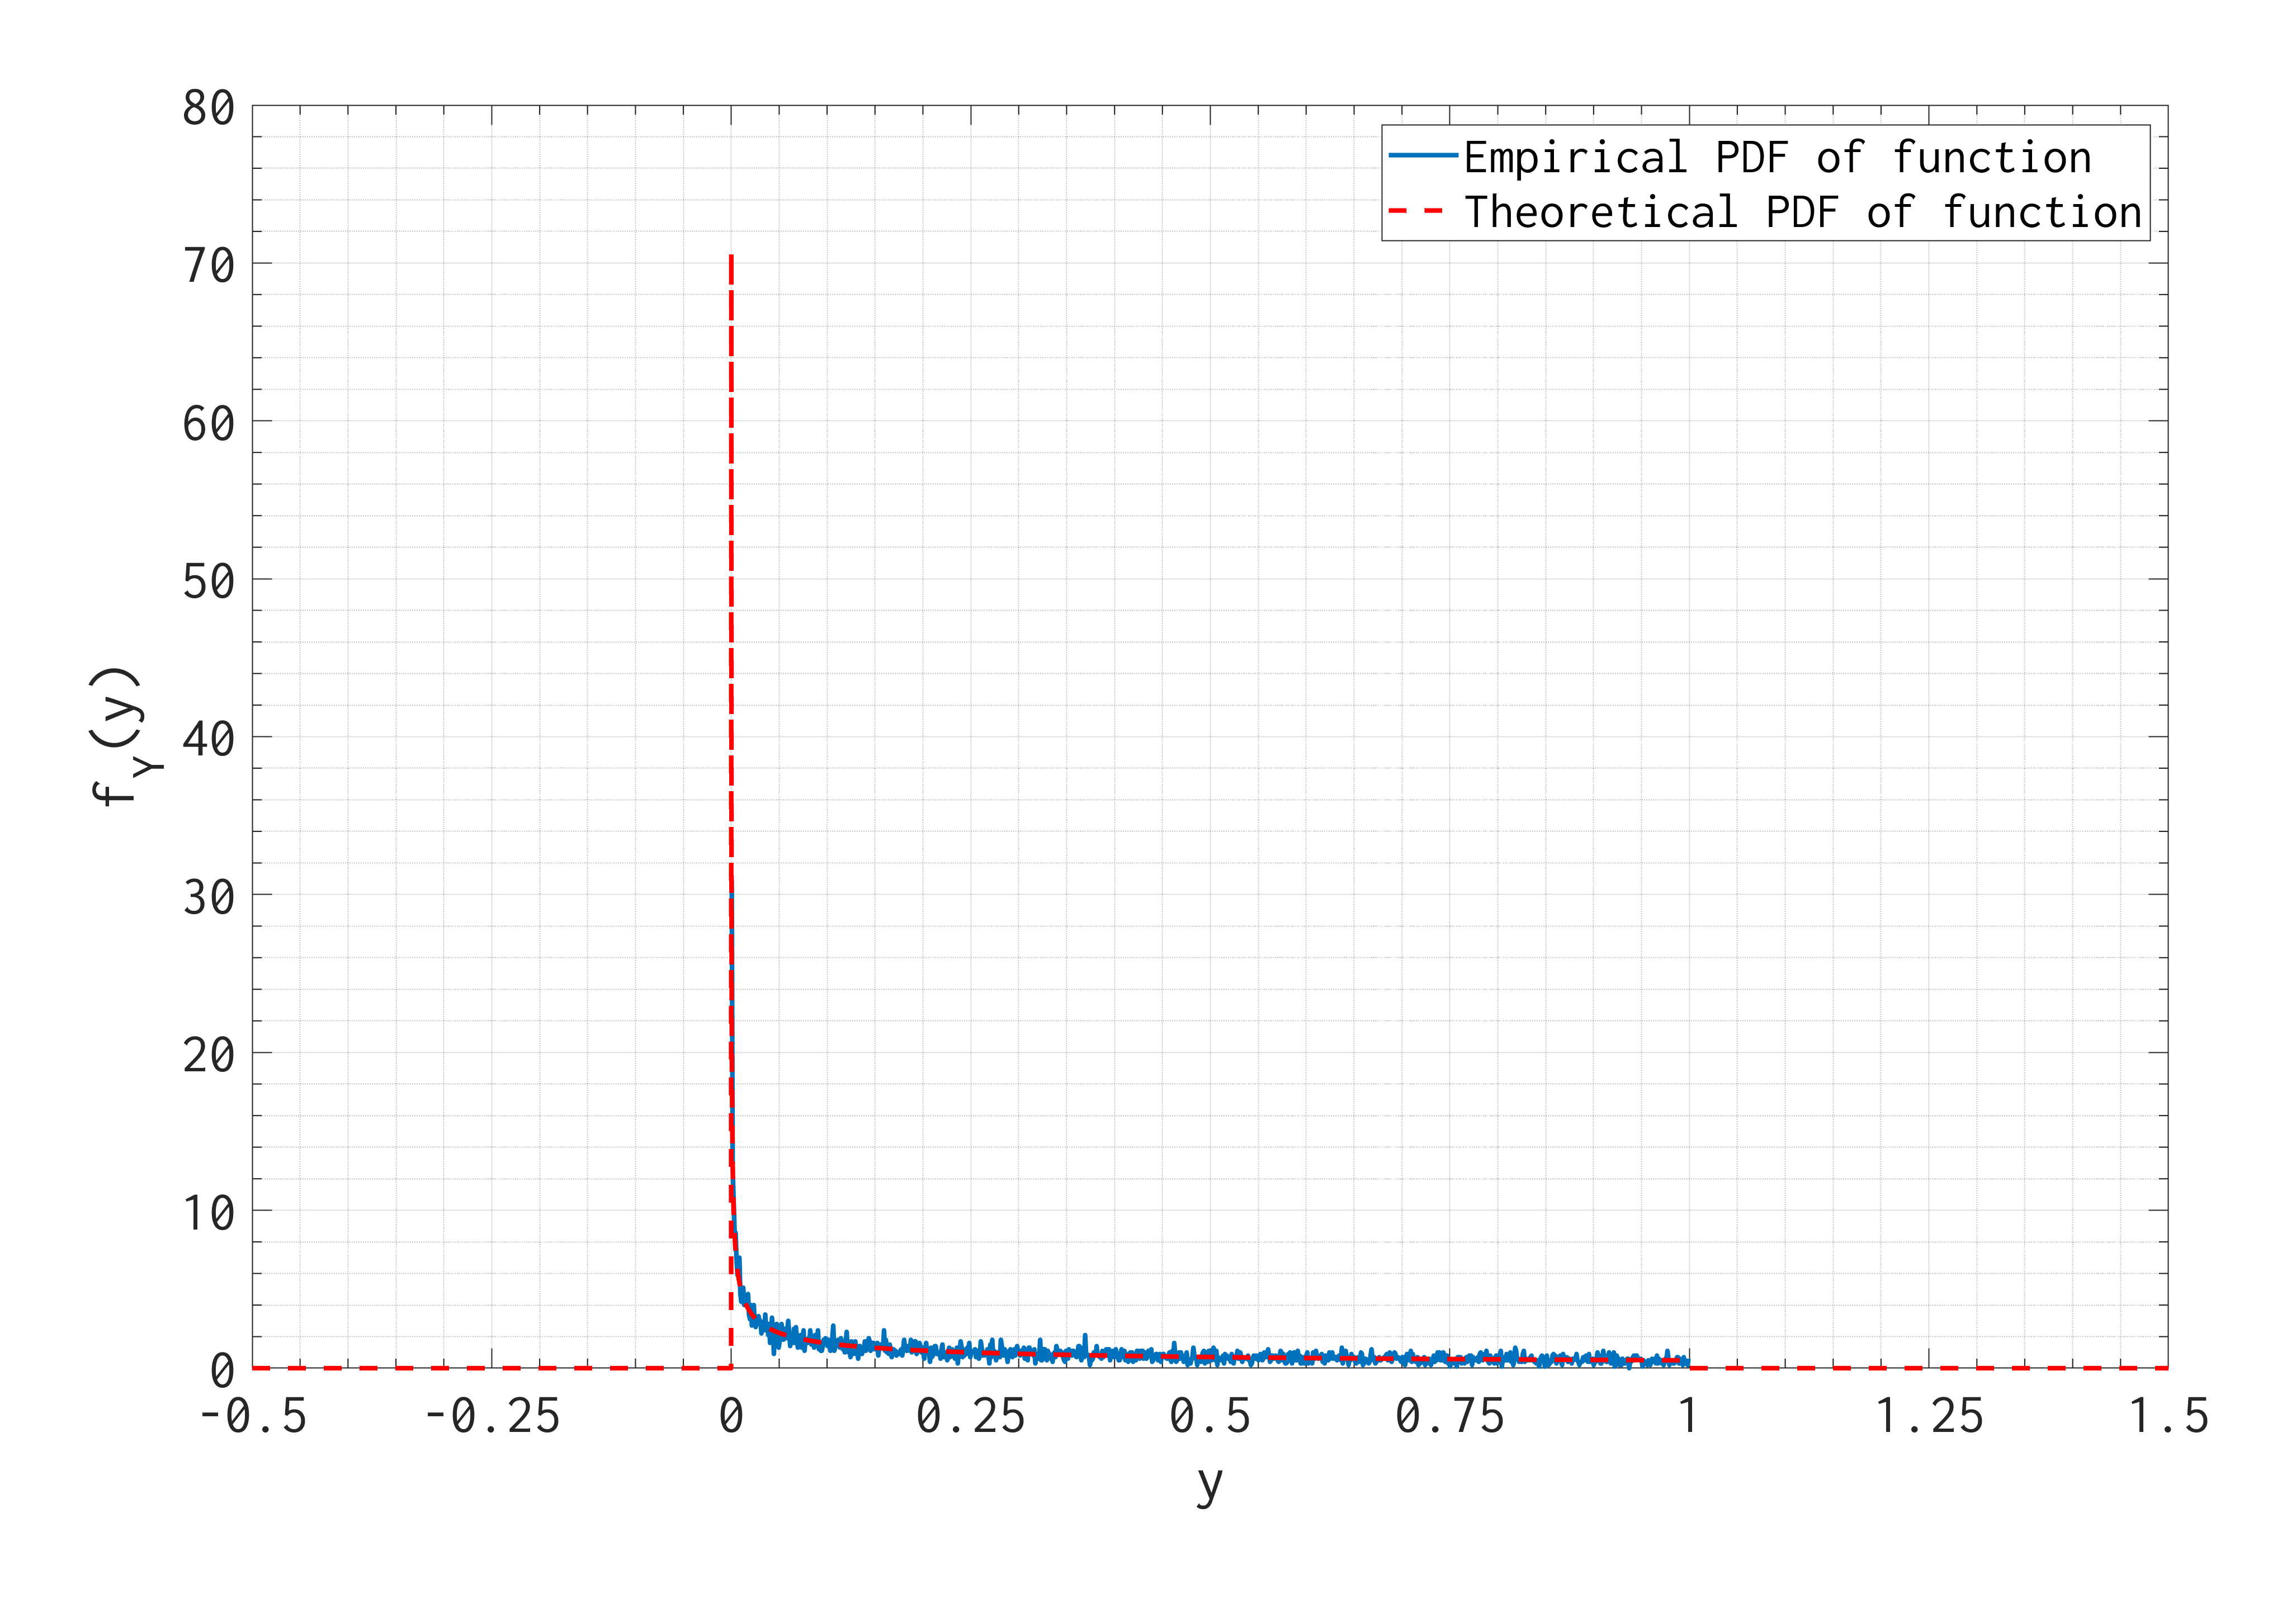
\includegraphics[scale=0.355]{figures/pdf_of_function.png}
    \caption{PDF Teórica e Empírica para o Exercício considerado.}
\end{figure}

\section{Cálculo de momentos de variáveis aleatórias}
Temos uma variável $X: S \rightarrow \bb{R}$ e uma função $g: \bb{R} \rightarrow \bb{R}$ que permite
definir a variável aleatória $Y = g(X)$.

Para calcularmos o valor esperado de $Y$ podemos usar a definição por meio do teorema do
\it{estatístico inconsciente} [\it{"inconscious statistician"}]
\begin{align*}
    E(Y) &= E(g(X)) \\
    E(y) &= \int^\infty_{-\infty} y \cdot f_y(y)dy = \mcolor{blue}{\int^\infty_{-\infty} g(x) \cdot
    f_X(x)dx} \\
\end{align*}

\it{Comentário:} Note que apesar da definição mostrar uma dependência pela PDF da função o teorema
mostra que não é preciso! Esse teorema pode ser generalizado e, em particular, no caso da variância
que ele gera uma notação importante (\bf{que não é um caso óbvio como a notação pode sugerir, mas
como consequência desse teorema})

\end{document}
